%************************************************
\chapter{Evaluation}\label{ch:evaluation}
%************************************************
This chapter evaluates the system proposed in \autoref{ch:design}. This evaluation is based on analysing the requirements that are described in \autoref{sec:architectural_req}. Furthermore, this chapter continues the evaluation of the proposed solution by means of an experimental procedure aimed at evaluating its accuracy. This chapter ends with answering the sub questions, as proposed in \autoref{sec:research_question}.

\section{Evaluating architectural requirements} \label{sec:eval_arch_req}
This section provides a small overview whether the architectural requirements are met. The numbering is consistent with the requirements in \autoref{sec:architectural_req}.

\begin{enumerate}
    \item The system has been designed in such a way that it is functional across multiple Cloud Providers. The system has been tested on Google Cloud Engine, while the case study operates on a private Cloud.
    \item The data transmitted between nodes is not secured, as it is being send over HTTP. However, the system should be set up in a way in which only the dashboard is publicly available. As this is the case, the data is only accessible in the Grafana dashboard. This can be seen only using a username-password authentication. However, the dashboard is automatically served over HTTP. Therefore, we conclude that the data is not secure.
    \item We conclude that the system is sufficient configurable. There are configuration options for all resource prices, network traffic monitoring and node types. Therefore, the system can be tweaked to support multiple systems, each with its own characteristics. However, this is not a full proof, and we verified the system only using a demo application and at an industrial company. The solution is easy to use, as it works without any configuration as well (due to default variables).
    \item \autoref{fig:deployment} presents the overhead of the monitoring solution during the case study. It shows that the overall CPU utilization is low. Furthermore, \autoref{sec:eval_k} explains how the solution can be tweaked to balance between efficiency and effectiveness. We conclude that there is a balance, although this must be configured.
    \item The solution is able to collect utilization statistics on the monitored system using cAdvisor and TCPdump, as described in \autoref{sec:node}.
    \item The proposed solution is scalable, although it has limits. Using the hierarchical structure defined in \autoref{sec:architecture}, the system is able to scale to tens of super nodes and millions of nodes. However, the data is not aggregated at the root, so this might become a bottleneck. The Grafana dashboard requests data from the Prometheus database, which returns each container with the corresponding info as a datapoint. As explained in the Grafana documentation \cite{grafana}, the maximum number of datapoints is $2495$. Therefore, we conclude that the proposed solution is not very scalable.
    \item The solution is elastic as it can detect new running containers and stopped containers. As a container is stopped and removed, the data persists in the database. Furthermore, in case of new resources (i.e. virtual machines) added to the system, the solution is able to automatically update the hierarchical structure (assuming the solution is configured correctly). If the new monitoring node is a supernode, than it automatically receives a number of nodes to monitor. If the new monitoring node is a normal node, it is automatically scraped by one of the available supernodes. Therefore, we conclude that the system is elastic.
    \item The solution is adaptable, as it can deal with spikes of network load. In this case, the monitoring solution has a smaller sleeping period, which leads to a decrease in the network sleeping time. However, this sleeping time is always a constant multiple of the network monitoring time. The solution is not affected by the load put on the system, as the monitored values are collected at regular intervals, which is independent of their value.
    \item The solution is not autonomic, as it is not able to self-manage its distributed resources by automatically reacting to unpredictable changes. Although the solution works by connecting a new monitoring node automatically to the other nodes, it cannot scale these nodes on-demand without the help of the Cloud Consumer. Therefore, we conclude that the system is not fully autonomic.
    \item The accuracy of the solution can be evaluated by determining the accuracy of the individual components. This is all described in the section below (\autoref{sec:accuracy_evaluation}). The conclusion of the accuracy evaluation can be found in \autoref{sec:accuracy_conclusion}.
\end{enumerate}

\noindent
From the items above, we conclude that the system is unsuccessful to meet all requirements. Three of them are not met, which are security, scalability and autonomicity. Six out of the other seven requirements are sufficiently met. The last requirement -accuracy- is evaluated in the section below.

\section{Accuracy evaluation} \label{sec:accuracy_evaluation}
The accuracy evaluation is divided into two parts. First, the accuracy of the pricing model proposed in \autoref{sec:pricing} can be found in \autoref{sec:eval_pricing}. Second, the accuracy of the network traffic monitoring can be found in \autoref{sec:eval_k}. Both evaluations are concluded in \autoref{sec:accuracy_conclusion}.

\subsection{Pricing model accuracy} \label{sec:eval_pricing}
Due to the complexity of the Cloud and a large number of Cloud Providers, it is not trivial to develop an accurate pricing model. This section evaluates the pricing model from \autoref{eq:p}. This pricing model is a combination of three price values, and three resource values.\\

\noindent
The price values are designed in such a way that they can be changed dynamically. Therefore, the user of the monitoring tool can adjust the prices such that they fit to his spendings. This provides a simple solution, but is based on the assumption that the prices do not change while monitoring the system (some Public Cloud Providers offers discount for longer use). Furthermore, it is also based on the assumption that there are no free resources when the deployment of the Cloud-based application is started (e.g. the first $50$ GB of outgoing network data is free). However, using the dynamic set up of this model, the issues mentioned above can be solved, by updating the prices. For example, if the price per outgoing GB is $\$0.10$, and the solution has monitored $200$ GB so far. The price for the model could be $\$0.075$ in case the first $50$ GB is indeed free. The same trick can be applied in case the Cloud Provider offers discount for longer use. However, by continuous changing the prices manually, we can conclude that the pricing model on itself is too simplistic and therefore limited accurate.\\

\noindent
It needs to be pointed out that the model, although simplistic, is easy-to-use. According to the technical employee of the industrial company, the ``pricing is of course configurable, so it can be adjusted to be more accurate for other scenarios''. Furthermore, the issues from the previous paragraph are only effective when the tool is used for at least a month. In \cite{infoworld} is explained that ``monthly usage, saves about $10$ percent over on-demand usage''. Therefore, its inaccuracy for monitoring two months is only $5\%$.\\

\noindent
The resource values are the network utilization, the CPU utilization and the memory utilization. The accuracy of the first is described in \autoref{sec:eval_k}, while the latter two are described in this section. In order to evaluate the accuracy of those two values in the system, a small architecture has been set up. This architecture consists of a demo system (two containers), an external cAdvisor for verification, and a supernode that monitors the resources of these two containers. The command for running this experiment is the following:

\begin{lstlisting}[language=bash, caption=Docker-compose]
git clone https://github.com/dadvisor/util
./util/utilization.sh
\end{lstlisting}

\noindent
After a few minutes, the results can be found on the Prometheus database of the supernode by using one of the following queries:

\begin{verbatim}
label_replace(rate(container_cpu_usage_seconds_total{id=~
"/docker/.*"}[5m]), "src", "$1", "id", "/docker/(.*)") / 
on (src) (rate(cpu_util_container_total[5m]) * 3600)

label_replace(container_memory_usage_bytes{id=~"/docker/.*"}
, "src", "$1", "id", "/docker/(.*)") / on (src)
(rate(mem_util_container_total[5m]) * 3600 * 
scalar(machine_memory_bytes))
\end{verbatim}

\noindent
The first query above is for the CPU analysis, while the second is for the memory analysis. The proposed solution uses a delay in getting the resource data, and it takes a delay before the data is scraped by the Prometheus database. The accuracy of the CPU utilization can be found in \autoref{fig:eval_cpu}. This figure shows that there is a difference of factor $4$ in the beginning, but later flattens out to $1$ (A value of $1$ corresponds to a perfect estimate.). The accuracy of the memory utilization can be found in \autoref{fig:eval_mem}. This figure shows the same pattern, except that the peak in the beginning is a bit higher.\\

\begin{figure}
    \centering
    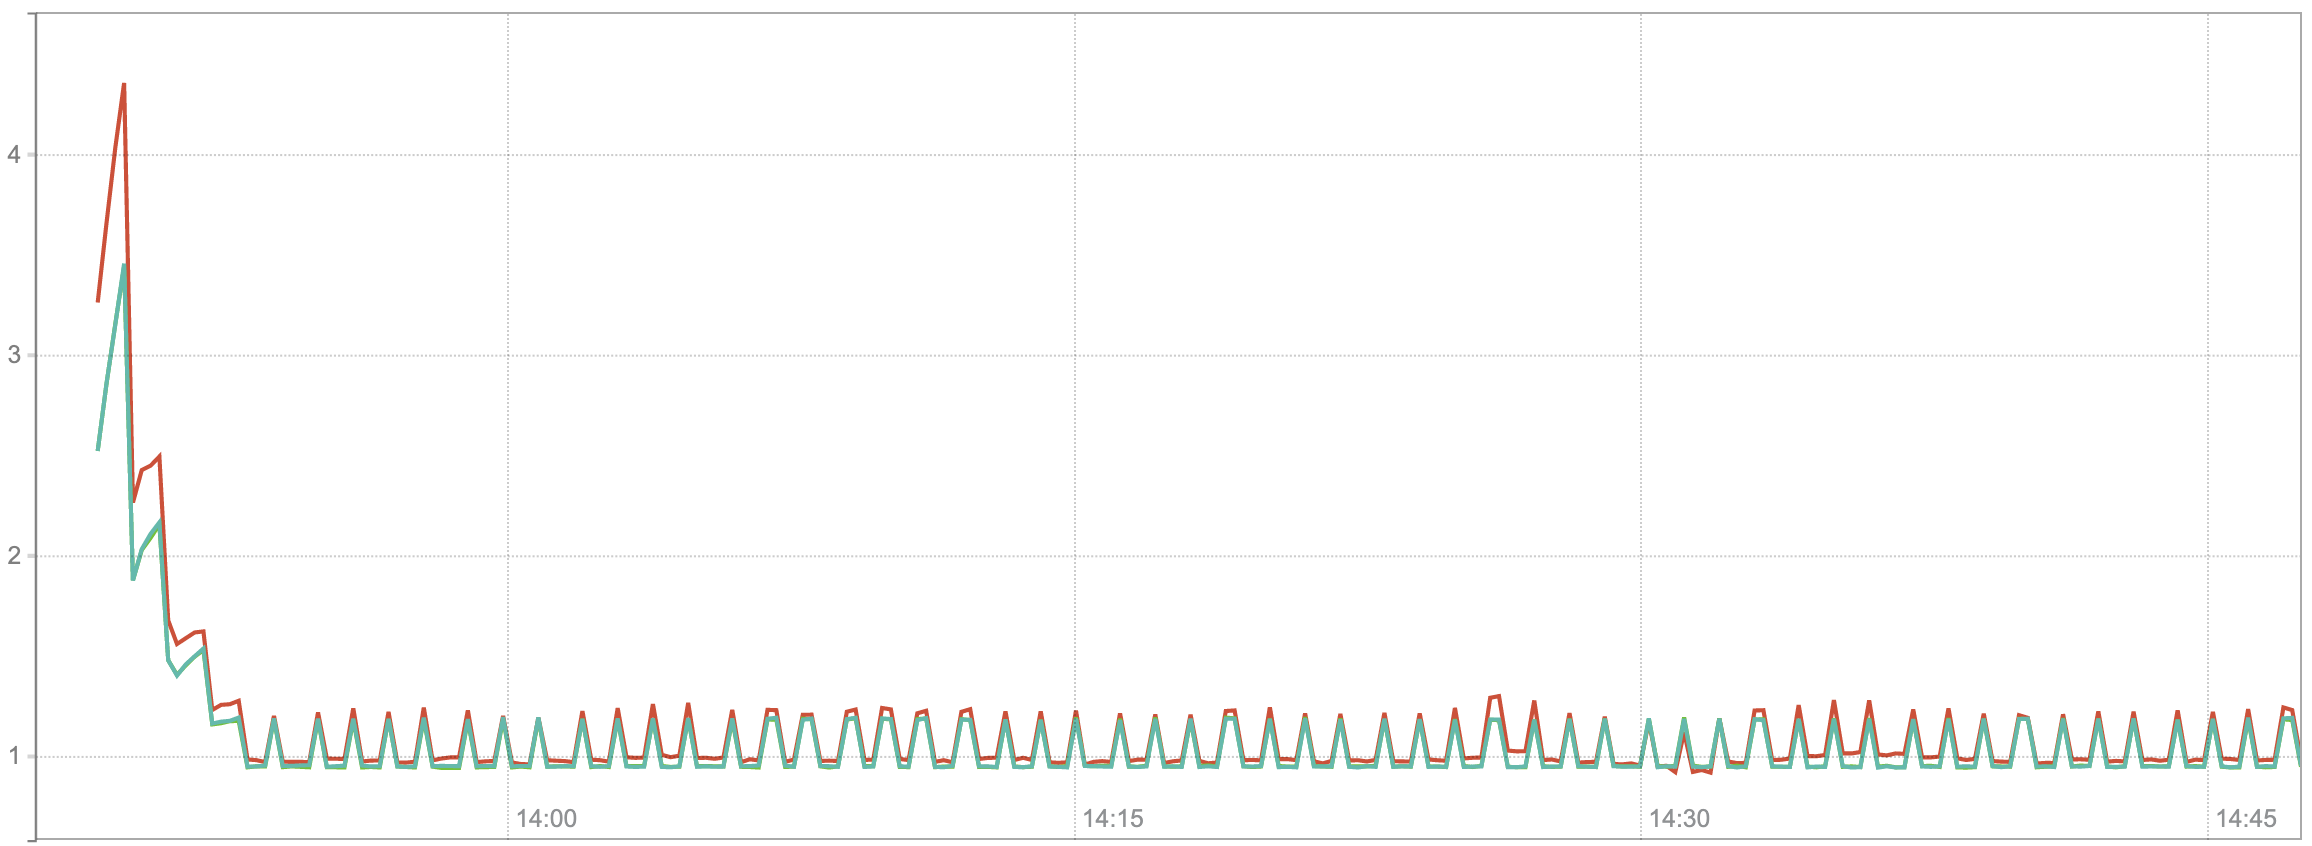
\includegraphics[width=\textwidth]{gfx/eval_cpu}
    \caption{Evaluation of the CPU accuracy}
    \label{fig:eval_cpu}
\end{figure}

\begin{figure}
    \centering
    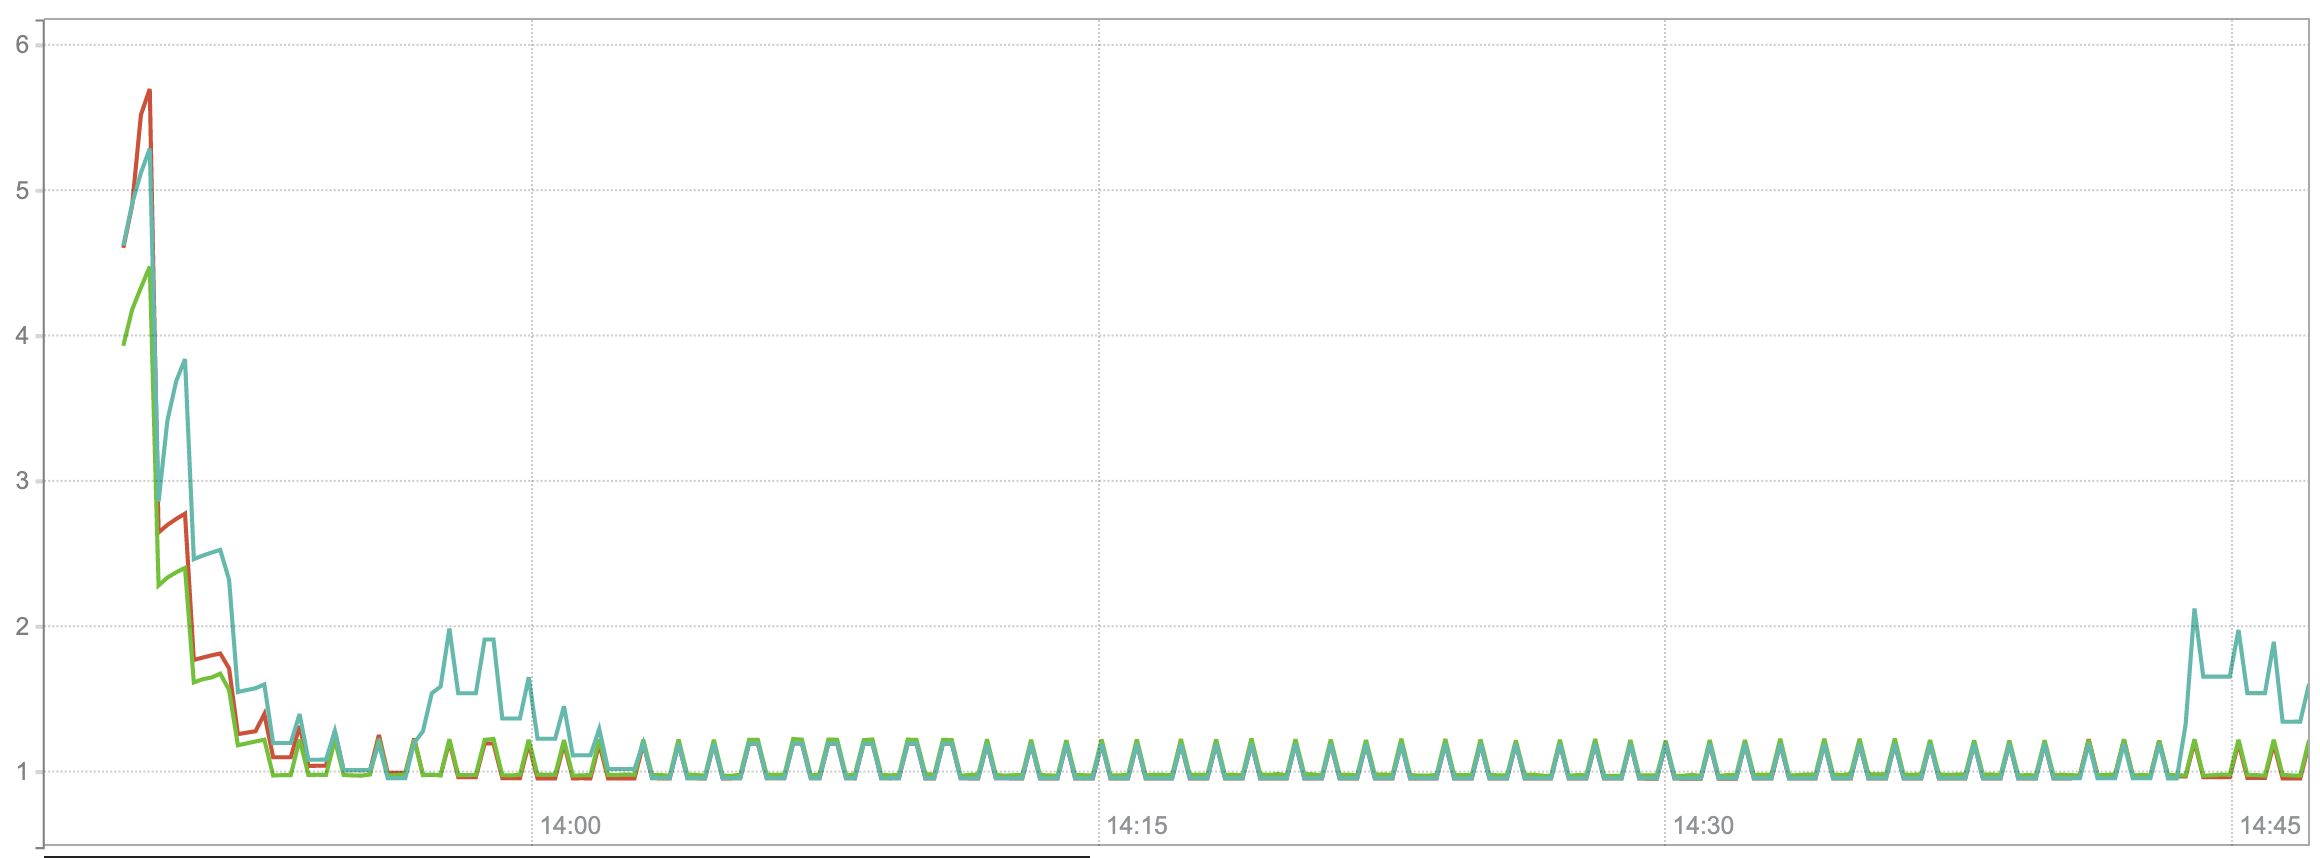
\includegraphics[width=\textwidth]{gfx/eval_mem}
    \caption{Evaluation of the Memory accuracy}
    \label{fig:eval_mem}
\end{figure}

\noindent 
We conclude that the pricing model is accurate to a certain extend. The latter of this section has shown that the utilization values are close to the real values, which makes them accurate. The first part of this section discusses the pricing values used. Although they are too simplistic, and therefore limited accurate, they provide an easy-to-use solution for the user of the tool.

\subsection{Network traffic accuracy} \label{sec:eval_k}
This section presents the accuracy of network traffic monitoring. In order to do so, a supernode was deployed to monitor two containers. One container acting as a web-service, and one container continuously sending requests. The command for collecting all values can be found below:

\begin{lstlisting}[language=bash, caption=Docker-compose]
git clone https://github.com/dadvisor/util
./util/accuracy.sh
\end{lstlisting}

\noindent
Using this system, there is only one container that communicates with the web-service. This implies that the total amount of data that the web-container sends is equivalent to its internal amount of data. Thus, the following variables should hold the same value:
\begin{itemize}
    \item \textbf{network\_container\_total}: This metric receives a value by scraping data from cAdvisor.
    \item \textbf{bytes\_send\_total}: This metrics has a key-value pair with both `src' and `dst'. This is the amount of data sent between the source container and the destination container by reading the TCPdump data.
\end{itemize}

\noindent
By analysing the rate (per-second average rate of increase) over a time period of one hour, the accuracy can be determined. This can be expressed as the ratio between the two variables above. A perfect estimation would therefore result in a value of $1$. The Prometheus query for analysing the accuracy is presented below.

\begin{verbatim}
rate(network_container_total[5m]) / on (src) 
rate(bytes_send_total[5m])
\end{verbatim}

\noindent
The analysis has been repeated for different K-values. The meaning of the K-values are described in \autoref{sec:exposing_data}. The data obtained for $K = 0$ can be found in \autoref{fig:network_traffic_accuracy}. This figure shows the accuracy of the network traffic monitoring evaluation. Note that this figure shows several spikes, which is due to the difference update frequency of both variables. Therefore, the minimum and maximum value represent the boundaries of the accuracy. Furthermore, the accuracy is summarized by computing the average. The accuracy is evaluated by an increasing load. The load for $K = 0$ can be found in \autoref{fig:increasing_load}. The results for different K-values can be found in \autoref{tab:accuracy_results}.

\begin{figure}
    \centering
    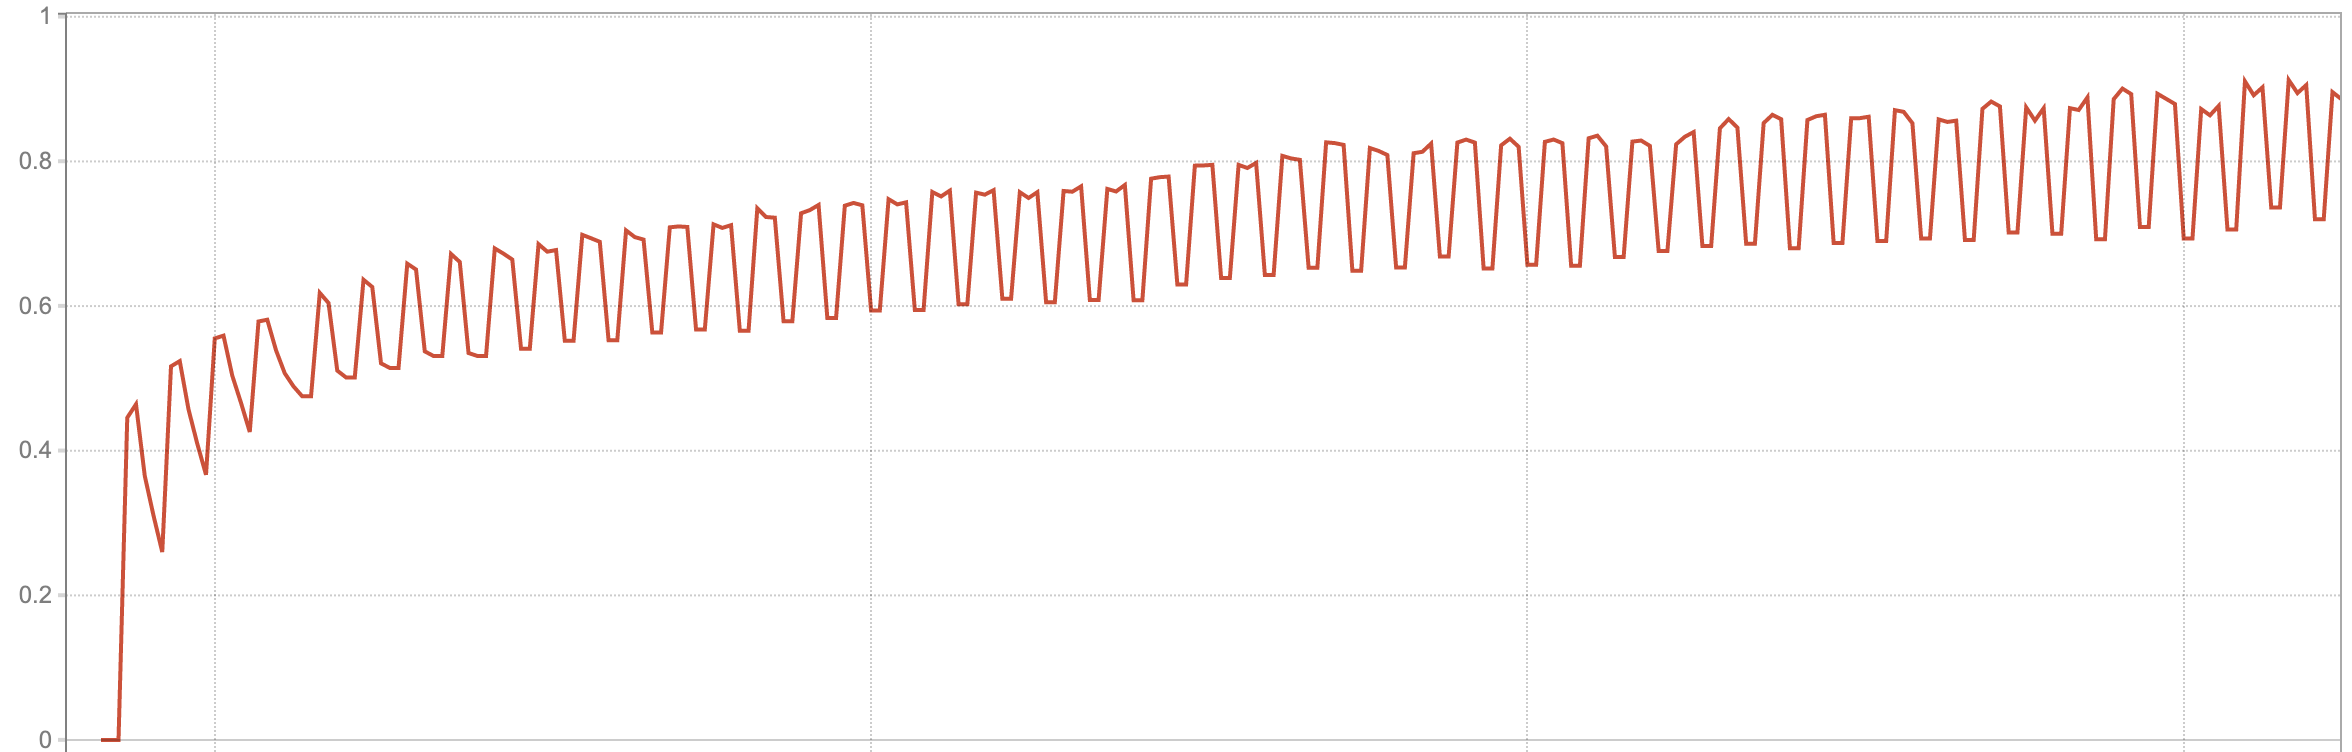
\includegraphics[width=\textwidth]{gfx/traffic_network_accuracy}
    \caption{Network traffic accuracy for $K = 0$}
    \label{fig:network_traffic_accuracy}
\end{figure}

\begin{figure}
    \centering
    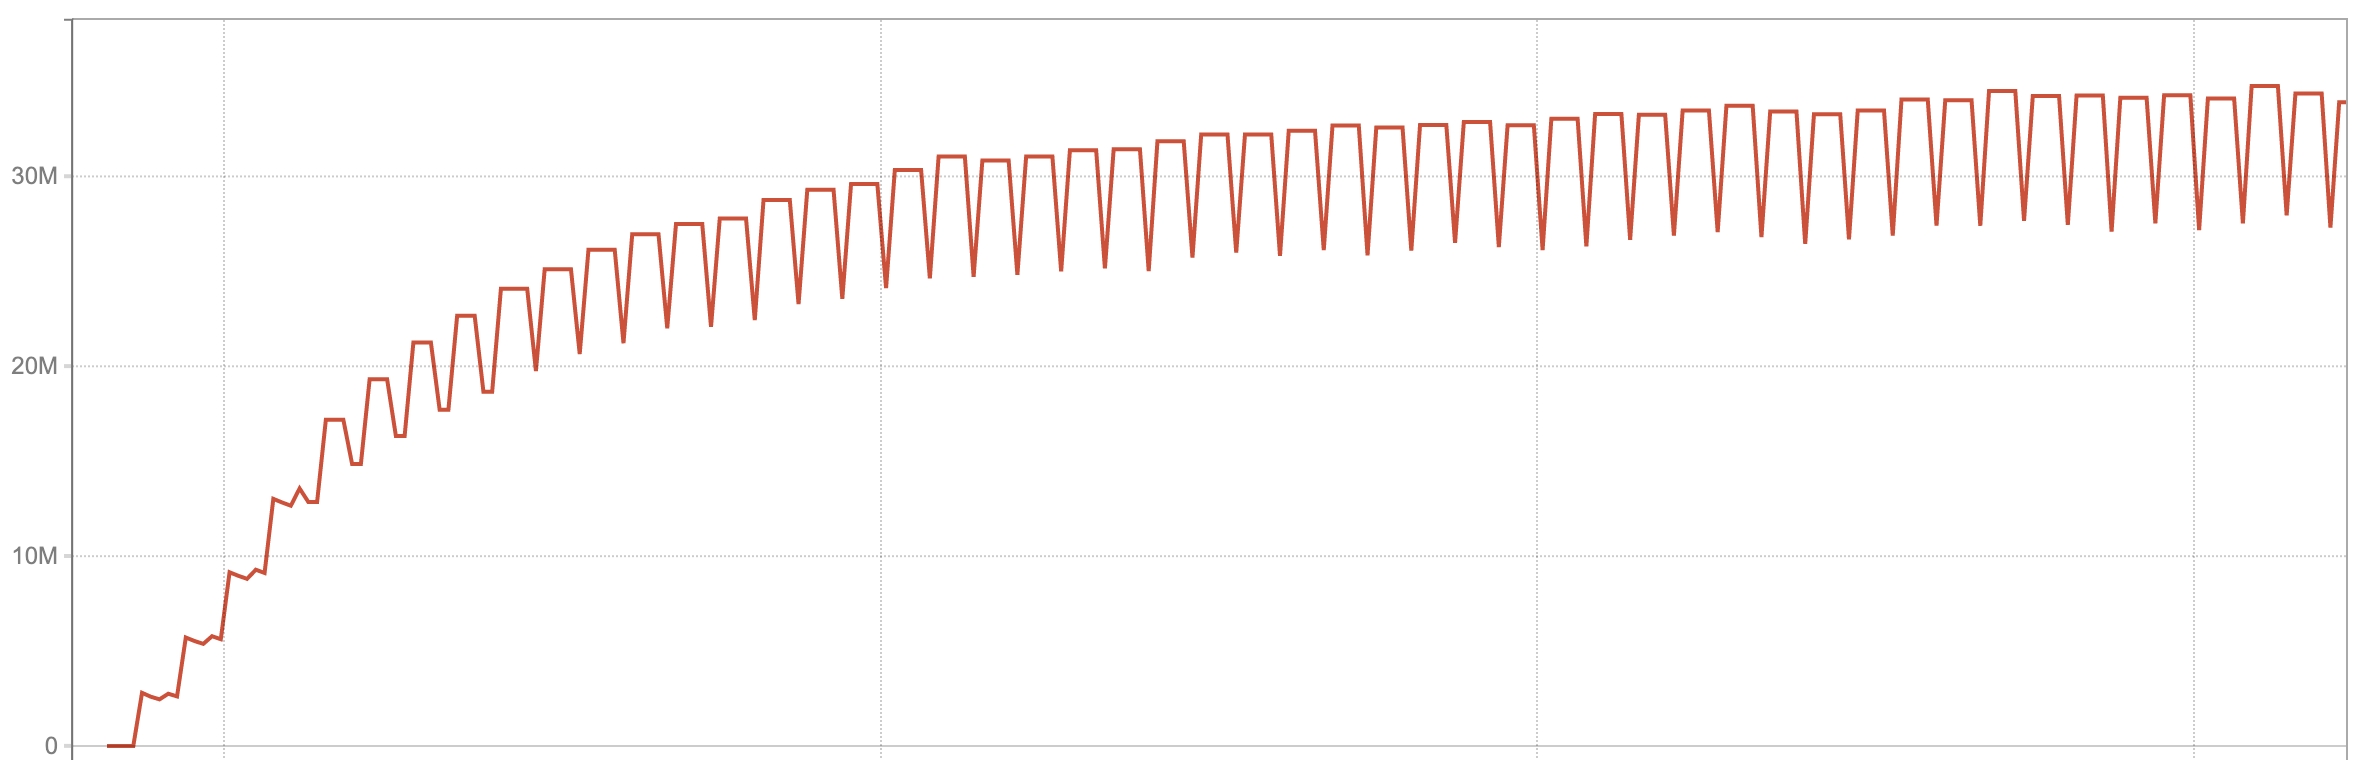
\includegraphics[width=\textwidth]{gfx/increasing_load}
    \caption{Simulating increasing load for $K = 0$}
    \label{fig:increasing_load}
\end{figure}

\begin{table}[ht]
    \centering
    \begin{tabular}{r|rrr|r}
        \multirow{2}{*}{K-value} & \multicolumn{3}{c|}{Accuracy} & \multirow{2}{*}{CPU Usage} \\
        & Min & Max & average & \\ \hline  
        0 & 0.26& 0.95& 0.77& 13\% \\
        3 & 0.22& 4.54& 2.43& 4\% \\
        6 & 0.20& 2.11& 0.75& 3\% \\
        9 & 0.24& 5.77& 2.31& 3\% \\
        12& 0.27& 3.50& 1.14& 2\% \\
        15& 0.20& 4.74& 1.40& 2\% \\        
    \end{tabular}
    \caption{Network traffic accuracy results for different K-values with increasing load}
    \label{tab:accuracy_results}
\end{table}

\subsection{Conclusion} \label{sec:accuracy_conclusion}
From \autoref{tab:accuracy_results} can be concluded that there is huge difference in average accuracy between the different K-values. Therefore, we cannot claim that the accuracy drops if the K-value increases. What can be concluded from this table, is the fact that the CPU usage drops if the K-value increases. This is due to a longer sleeping period. However, this number is not very accurate, as the analyses is performed on a single node. Therefore, the overhead of communicating with other nodes is not evaluated.

\section{Evaluating sub questions} \label{sec:subquestions}
This section evaluates the sub questions proposed in \autoref{sec:research_question}. The research question (\textbf{Q1}) is answered in \autoref{ch:conclusion}.

\begin{quote}
    \begin{itemize}
        \item[\textbf{Q2}: ]\textit{How can the utilization of a Cloud-based application be monitored in an effective manner?}
    \end{itemize}
\end{quote}
\noindent
The utilization of a Cloud-based Application is monitored using the proposed solution, which is running on every Virtual Machine of the system. The solution consists of the cAdvisor monitoring tool and the own developed dAdvisor. The latter aggregates the information from cAdvisor, and exports it to Prometheus. This is configured such that it strives a balance between effectiveness and efficiency by aggregating the data every minute. Therefore, the proposed solution has limited accuracy (as can be seen in \autoref{fig:eval_cpu} and \autoref{fig:eval_mem}).


\begin{quote}
    \begin{itemize}
        \item[\textbf{Q3}: ]\textit{What is an accurate pricing model for estimating the cost of a Cloud-based application?}
    \end{itemize}
\end{quote}
\noindent
The pricing model used in this thesis is described in \autoref{sec:pricing}. It is evaluated in \autoref{sec:eval_pricing}. From the evaluation it becomes clear that the pricing model adopted is too simplistic and therefore it has limited accuracy. This becomes clear when the pricing model is used for a period of at least two months\footnote{This is explained in \autoref{sec:eval_pricing}.}. On the other hand, the model is flexible, allowing easy changes of the pricing values used. Therefore, we conclude that the pricing model fits for the case study with the industrial company, and provides an easy-to-use model for the proposed solution.


\begin{quote}
    \begin{itemize}
        \item[\textbf{Q4}: ]\textit{What is an effective approach for computing the waste of a Cloud-based application?}
    \end{itemize}
\end{quote}
\noindent
In \autoref{sec:approaches}, three approaches are designed to distribute the unused resources over the available containers. These approaches are first evaluated in \autoref{sec:optimal_approach} by their memory and computational complexity. Furthermore, they are evaluated by the accuracy, which is interpreted as which approach divides the waste using a fair distribution. This leads to an effective approach, which is described in \autoref{sec:linear}.

\begin{quote}
    \begin{itemize}
        \item[\textbf{Q5}: ]\textit{How can the cost and waste be presented to the user in a scalable and effective manner?}
    \end{itemize}
\end{quote}
\noindent
In order to answer this sub question, the question can be divided into two parts. First, the scalability is already discussed in \autoref{sec:eval_arch_req}. This section explains that the presented info is scalable, but has it limits. Effectiveness is evaluated by the CPU usage, as presented in \autoref{tab:accuracy_results}. This table shows that the overhead is quite low, depending on the K-value used. Using the case study, we determine the overhead of running the root node. \autoref{fig:deployment:jotunheim-root} shows that the average CPU utilization is $2.5\%$. This implies that the data is presented in an effective manner. 

\section{Conclusion}
This chapter has provided the evaluation of the system. We conclude that most requirements are met, with seven out of ten. The accuracy of the system is evaluated in \autoref{sec:accuracy_evaluation}. This section concludes that the pricing model is not completely accurate, and the network accuracy is sufficient accurate for $K = 0$. This chapter ends with answering the sub questions in \autoref{sec:subquestions}. The sub questions are used for answering the research question in \autoref{ch:conclusion}.